\section{x-commerce overview}
\label{sec:x_commerce_overview}
X-commerce is a web platform for building e-commerce systems. This platform build full-stack Javascript NodeJS API-centric HTML5 based Single Page Application with Web Components via Polymer-Project. In particular, the core of x-commerce follows the philosophy of Polymer project or all the complex parts of the platform are self-contained and isolated so that the responsibilities are well localized. In other words, x-commerce has been developed to facilitate the modifiability of the code, integrity of new services and reusability. This is facilitated, thanks to Polymer for which: “Everything is an element, even a service.”
So, a Web platform is essentially built by composing elements together.
\newline
For example a page of a product has been divided into various elements and each element contributes to realize the same page. In this way any changes related to the code are very well located. In following it is, a more abstract level designed as a page in general.
\begin{figure}[htb]
 \centering
 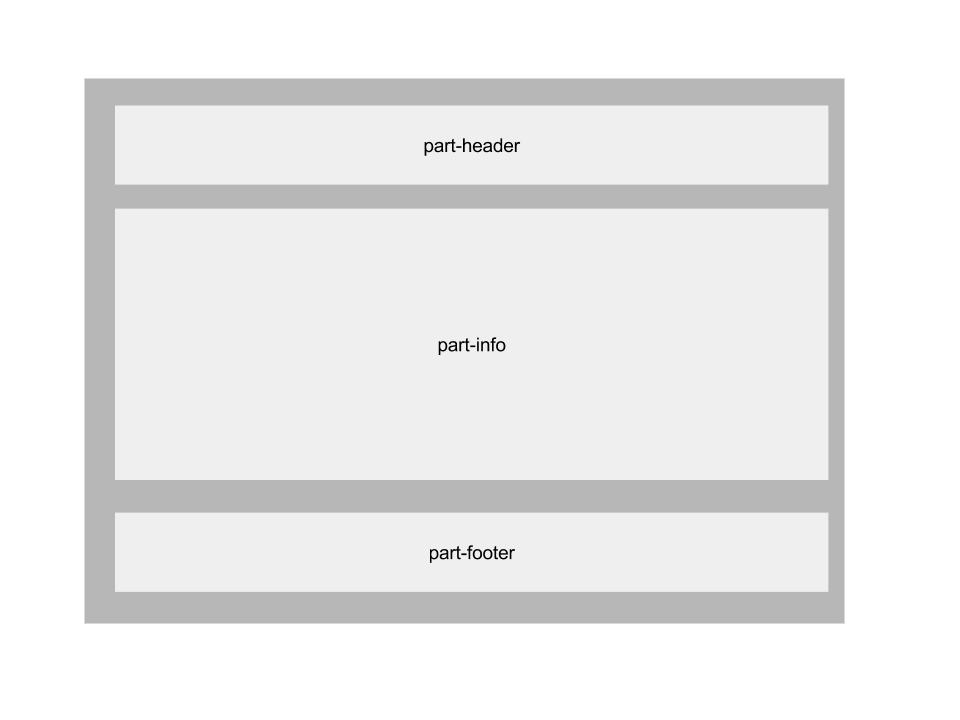
\includegraphics[width=1.0\linewidth]{images/chapter4/design-page.jpg}\hfill
 \caption[Design page]{Example of how the pages are designed}
 \label{fig:design_page}
\end{figure}
So e-commerce is a platform developed for composition of elements. This philosophy also aids code reusability. In fact, in the navigation of web pages, between the previous and the next, there is a lot in common, such as header and footer. With the Web components, the elements that are often used by most parties are also created.
Moreover, with help of the Web Components philosophy, it’s easy to gain a clear separation between structure, content, behavior and presentation of elements. It is possible to create components that are related only to the presentation part of an element, such as mixins in which developers can express groups of CSS rules to be applied to different elements.
\newline
On a small project, the potential of Polymer may not be very obvious, but when the project is large the philosophy that “everything is an element” helps a lot in design and construction.